%!TeX root = main.tex
%!encoding = UTF-8 Unicode
\section{EMC in Power Electronics}

Electromagnetic compatibility (EMC) describes the ability of electrical and electronic equipment to operate in an electromagnetic environment as intended without causing or experiencing unacceptable interference. 
An EMC problem generally involves three elements: a noise source, a propagation path, and a noise sink. 
The noise source generates electromagnetic disturbances, the propagation path transfers them through conducted or radiated coupling, and the sink responds to the resulting disturbance. 
\fref{fig:BlockDiagram_SourceVictim} illustrates this model with a measurement port in the propagation path.
The port can be used to measure disturbances from the source or to inject a defined disturbance for an immunity test of the sink.
\begin{figure}
	\centering\import{./figures/2_Fundamentals/}{BlockDiagram_SourceVictim.pdf_tex}
	\caption{Block diagram of EM interaction between source, propagation path, and sink.}
	\label{fig:BlockDiagram_SourceVictim}
\end{figure}

In a power-electronic converter, the switching semiconductor devices are the dominant noise sources, while the converter layout, passive components, cables, and enclosure determine the available propagation paths. 
Other circuits or sensors connected to, or located near, the converter may act as victims.
This situation is particularly relevant in electric vehicles, where high-power inverters are located close to sensitive electronic components and sensors, such as those used for safety applications and autonomous-driving systems.

\FloatBarrier

\subsection{Emission Generation}
\label{sec:Fundamental_Generation}
The fast voltage and current transients produced by switching power-semiconductor devices excite electromagnetic disturbances in the surrounding circuit.
Following the graphical approach presented by Costa~\cite{costa_graphical_2005}, the analysis starts with a periodic rectangular pulse and then introduces finite transition times, waveform asymmetry, and resonance.
Gaussian smoothing provides a theoretical reference for spectral concentration, while a simulated waveform illustrates the combined effects and the need for experimental validation.
The analysis concerns the switching-voltage spectrum at the source, rather than the emissions at a system port.

\subsubsection*{Rectangular-Pulse Spectrum}
\textbf{Isolated Pulse:} A rectangular pulse provides the simplest representation of a switching waveform and serves as the starting point for the analysis:

\begin{equation}
	s(t) = \mi{V}{DC}\cdot\text{rect}\left(\frac{t}{\text{d}\mi{T}{s}}\right), 
\end{equation}
where \mi{V}{DC} is the DC-link voltage, $\text{d}$ is the duty cycle, and \mi{T}{s} is the switching period.
Using the Fourier-transform convention with kernel $e^{-j2\pi ft}$ gives
\begin{equation}
	S(f) = \mi{V}{DC}\cdot\text{d}\mi{T}{s}\cdot\text{si}\left(\pi f\text{d}\mi{T}{s}\right),
\end{equation}
where $\text{si}(x) = \sin(x)/x$ and $\text{si}(0) = 1$.
Because the Fourier transform integrates voltage over time, $S(f)$ has units of voltage multiplied by time. It describes the continuous spectrum of one isolated pulse; voltage-valued Fourier-series coefficients arise when the pulse is repeated periodically, as described next.

\textbf{Periodic Pulse Chain:} To represent steady-state switching, the isolated pulse is repeated at the switching period by convolution with a Dirac comb, forming a periodic pulse chain (PC):
\begin{equation}
	\mi{s}{PC}(t) = s(t) * \sum_{n=-\infty}^{\infty} \delta(t-\text{n}\mi{T}{s}).
\end{equation}
With $\mi{f}{s} = 1/\mi{T}{s}$, its Fourier transform becomes
\begin{equation}
	\mi{S}{PC}(f) = \sum_{n=-\infty}^{\infty} \frac{S(\text{n}\mi{f}{s})}{\mi{T}{s}}\,\delta(f-\text{n}\mi{f}{s}).
\end{equation}
Periodic repetition thus produces discrete spectral lines at integer multiples of the switching frequency.
For harmonic order $n$, the complex Fourier-series coefficient is $S(\text{n}\mi{f}{s})/\mi{T}{s}$.
Its magnitude is given by the continuous two-sided coefficient envelope evaluated at that harmonic:
\begin{equation}
A(f) = \frac{|S(f)|}{\mi{T}{s}}.
\end{equation}


\textbf{Spectral Envelope:} Logarithmic frequency and decibel voltage scales facilitate comparison of EMC spectra spanning several orders of magnitude.
Accordingly, the two-sided coefficient envelope $A(f)$ is expressed in logarithmic form relative to a voltage reference \mi{V}{ref}:
\begin{equation}
A_\text{dB}(f) = 20\log_{10}\left(\frac{A(f)}{\mi{V}{ref}}\right).
\end{equation}
The reference $\mi{V}{ref} = \SI{1}{\micro\volt}$ gives levels in dB\textmu V.
Here, $A(f)$ denotes a two-sided Fourier-series coefficient magnitude, not a single-sided peak or RMS amplitude.
For a real waveform, the corresponding nonzero harmonic has peak amplitude $2A(n\mi{f}{s})$ and RMS amplitude $\sqrt{2}A(n\mi{f}{s})$.
This normalization must be accounted for when comparing the analytical envelope with FFT results or receiver readings.

For the rectangular pulse shown in \fref{fig:Diss_SpectrumCreation_zeroOrder}, the low-frequency asymptote is the DC coefficient $\text{d}\mi{V}{DC}$, while the high-frequency envelope decreases in proportion to $1/f$, corresponding to a \SI{-20}{dB/dec} slope in a logarithmic plot.
The intersection of these asymptotes defines the first corner frequency:
\begin{equation}
	\mi{f}{c1} = \frac{1}{\pi\text{d}\mi{T}{s}}.
\end{equation}
This corner frequency is an intersection of asymptotes, not a sharp transition in the exact si-function spectrum.

\begin{figure}[h]
	\centering
	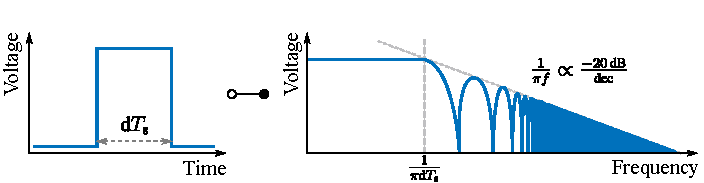
\includegraphics[scale = 1]{figures/2_Fundamentals/Diss_SpectrumCreation_zeroOrder.pdf}
	\caption{Graphical representation of the creation of the emission spectrum from a zero-order approximation of the switching transient.}
	\label{fig:Diss_SpectrumCreation_zeroOrder}
\end{figure}
\FloatBarrier


\subsubsection*{Influence of the Transition Shape}
\textbf{Equal Rise and Fall Times:} The rectangular approximation neglects the finite switching speed of real semiconductor devices.
Introducing linear transitions of equal duration \mi{t}{r} gives a trapezoidal pulse, obtained by convolving the rectangular pulse with a unit-area rectangular smoothing kernel:
\begin{equation}
	s(t) = \mi{V}{DC}\cdot\text{rect}\left(\frac{t}{\text{d}\mi{T}{s}}\right) *\frac{1}{\mi{t}{r}} \text{rect}\left(\frac{t}{\mi{t}{r}}\right).
\end{equation}
The convolution smooths the switching edges while preserving the pulse area.
Convolution in the time domain corresponds to multiplication in the frequency domain:
\begin{equation}
	S(f) = \mi{V}{DC}\cdot\text{d}\mi{T}{s}\cdot\text{si}\left(\pi f\text{d}\mi{T}{s}\right) \cdot \text{si}\left(\pi f \mi{t}{r}\right).
\end{equation}
The second si factor introduces an additional corner frequency,
\begin{equation}
	\mi{f}{c2} = \frac{1}{\pi\mi{t}{r}}.
\end{equation}
For $\mi{t}{r} \ll \text{d}\mi{T}{s}$, the envelope has three distinct regions: an approximately constant low-frequency region, a \SI{-20}{dB/dec} region, and a \SI{-40}{dB/dec} region above \mi{f}{c2}.
As illustrated in \fref{fig:Diss_SpectrumCreation_firstOrder}, the pulse duration and transition duration therefore control different parts of the envelope: the former sets the first corner, while the latter determines the onset of the additional high-frequency attenuation.

\begin{figure}[h]
	\centering
	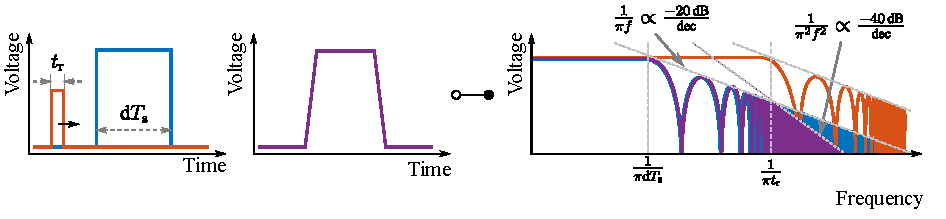
\includegraphics[scale = 1]{figures/2_Fundamentals/Diss_SpectrumCreation_firstOrder.pdf}
	\caption{Graphical representation of the creation of the emission spectrum from a first-order approximation of the switching transient.}
	\label{fig:Diss_SpectrumCreation_firstOrder}
\end{figure}

\textbf{Unequal Rise and Fall Times:}
Power-semiconductor devices generally exhibit different switching speeds during turn-on and turn-off, resulting in unequal rise and fall times.
To account for this asymmetry, the convolution-based approximation introduces separate transition-shaping terms for the rising and falling edges, as illustrated in \fref{fig:Diss_SpectrumCreation_asymTr}:
\begin{equation}
	s(t) = \mi{V}{DC} \cdot \text{rect}\left(\frac{t}{\text{d}\mi{T}{s}}\right) * \left(\mi{s}{sw,r} + \mi{s}{sw,f}\right)
\end{equation}
where \mi{s}{sw,r} and \mi{s}{sw,f} represent the respective transition-shaping terms.
In the graphical spectral approximation, the corresponding contributions are expressed as the sum of two si~functions:
\begin{equation}
	S(f) = \mi{V}{DC}\cdot\text{d}\mi{T}{s}\cdot\text{si}\left(\pi f\text{d}\mi{T}{s}\right) \cdot \left(\text{si}\left(\pi f \mi{t}{r}\right) + \text{si}\left(\pi f \mi{t}{f}\right)\right)
\end{equation}

The two transition durations introduce distinct corner frequencies, $1/(\pi\mi{t}{r})$ and $1/(\pi\mi{t}{f})$.
The longer transition begins to attenuate its spectral contribution at a lower frequency, allowing the faster edge to dominate between the two corners.
Above both corners, the asymptotic envelope decreases again at \SI{-40}{dB/dec}.

\begin{figure}[h]
	\centering
	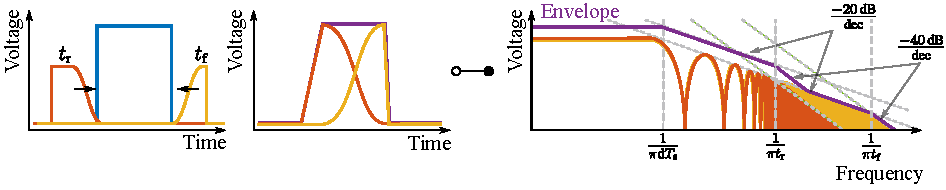
\includegraphics[scale = 1]{figures/2_Fundamentals/Diss_SpectrumCreation_asymTr.pdf}
	\caption{Switching waveform and spectral envelope for unequal rise and fall times.}
	\label{fig:Diss_SpectrumCreation_asymTr}
\end{figure}
\FloatBarrier

\textbf{Two-Slope Transitions:}
Whereas the preceding approximation distinguishes the rising and falling edges, a two-slope approximation accounts for changes in slope within an individual transition.
During turn-on, for example, the initial drain-source voltage change is influenced by the commutation-loop inductance and the current rise, while the subsequent voltage fall is governed by the gate drive and device capacitances.
This behavior is represented by convolving the rectangular pulse with the sum of two rectangular smoothing functions of different durations, as illustrated in \fref{fig:Diss_SpectrumCreation_twoTr}:
\begin{equation}
	s(t) = \mi{V}{DC} \cdot \text{rect}\left(\frac{t}{\text{d}\mi{T}{s}}\right) * \left(\frac{1}{\mi{t}{r1}} \text{rect}\left(\frac{t}{\mi{t}{r1}}\right) + \frac{1}{\mi{t}{r2}} \text{rect}\left(\frac{t}{\mi{t}{r2}}\right)\right)
\end{equation}
The corresponding frequency-domain expression is
\begin{equation}
	S(f) = \mi{V}{DC}\cdot\text{d}\mi{T}{s}\cdot\text{si}\left(\pi f\text{d}\mi{T}{s}\right) \cdot \left(\text{si}\left(\pi f \mi{t}{r1}\right) + \text{si}\left(\pi f \mi{t}{r2}\right)\right)
\end{equation}

This expression has the same mathematical form as the preceding graphical approximation, but the two durations now characterize contributions within a switching edge rather than separate rising and falling edges.

\begin{figure}[h]
	\centering
	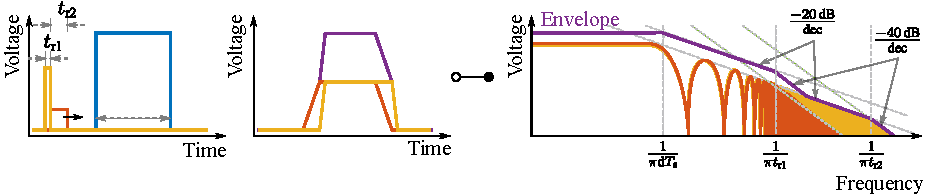
\includegraphics[scale = 1]{figures/2_Fundamentals/Diss_SpectrumCreation_twoTr.pdf}
	\caption{Switching waveform and spectral envelope for a two-slope transition approximation.}
	\label{fig:Diss_SpectrumCreation_twoTr}
\end{figure}
\FloatBarrier

\subsubsection*{Resonant Contributions}
Whereas the preceding models describe monotonic transitions, practical switching waveforms often exhibit overshoot followed by damped oscillations.
The underlying resonances arise from the interaction between the commutation-loop inductance and the output capacitance of the device in the off state.
Their excitation adds spectral contributions at the resonance frequencies, with the magnitude and width governed by the excitation strength and damping.
Differences in the effective capacitances and circuit conditions during turn-on and turn-off can produce distinct oscillation frequencies \mi{f}{on} and \mi{f}{off}, as modeled and predicted in~\cite{xu} and observed in the measurements presented in this thesis.
\fref{fig:Diss_SpectrumCreation_res} illustrates the resulting modification of the switching-edge spectrum.
\begin{figure}[h]
	\centering
	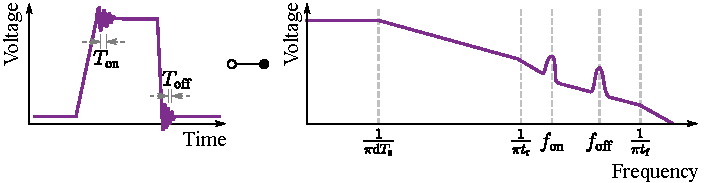
\includegraphics[scale = 1]{figures/2_Fundamentals/Diss_SpectrumCreation_res.pdf}
	\caption{Graphical representation of the creation of the emission spectrum from a resonant approximation of the switching transient.}
	\label{fig:Diss_SpectrumCreation_res}
\end{figure}

Taken together, the transition and resonance models explain individual features of the spectrum without reproducing the complete switching process.
Voltage-dependent capacitances and interactions between the gate and power circuits further modify the waveform, limiting the quantitative accuracy of these idealized representations.

\subsubsection*{Gaussian Smoothing as a Theoretical Reference}
Transition duration alone does not determine high-frequency emissions; waveform smoothness also affects spectral decay. 
Piecewise-linear transitions have discontinuities in their first derivatives, giving a high-frequency spectrum that decays in proportion to \SI{-40}{dB/dec}.
For comparison, convolution with a Gaussian kernel produces an infinitely differentiable ($C^\infty$) waveform, which can be expressed as:
\begin{equation}
	s(t) = \mi{V}{DC} \cdot \text{rect}\left(\frac{t}{\text{d}\mi{T}{s}}\right) * \left(\frac{1}{\sqrt{2\pi}\sigma_t}e^{-\frac{t^2}{2\sigma_t^2}}\right),
\end{equation}
where $\sigma_t$ is the standard deviation of the smoothing kernel.
Its Fourier transform yields
\begin{equation}
	S(f) = \mi{V}{DC} \cdot \text{d}\mi{T}{s} \cdot \text{si}(\pi f\text{d}\mi{T}{s}) \cdot e^{-(2\pi\sigma_t f)^2}.
\end{equation}
The Gaussian factor causes increasingly strong attenuation as frequency rises, so its envelope curves downward on a logarithmic-frequency plot instead of following a constant dB/decade slope, as illustrated in \fref{fig:Diss_SpectrumCreation_Heisenberg}:
For RMS measures of temporal and spectral width, the Gaussian kernel minimizes their product (the Heisenberg-Gabor limit) and thus provides a theoretical reference for minimizing spectral spread at a given temporal spread~\cite{signal_theory}.
Patin introduced this Gaussian waveform as the EM-noise-optimal switching waveform~\cite{Patin_HeisenbergGabor}.
In a power device, however, such a smooth, extended transition would be critical, since it prolongs the interval during which high voltage and high current are both present in the device, raising switching losses drastically.
The Gaussian waveform is therefore a theoretical benchmark; practical designs must balance spectral attenuation against switching loss.

\begin{figure}[h]
	\centering
	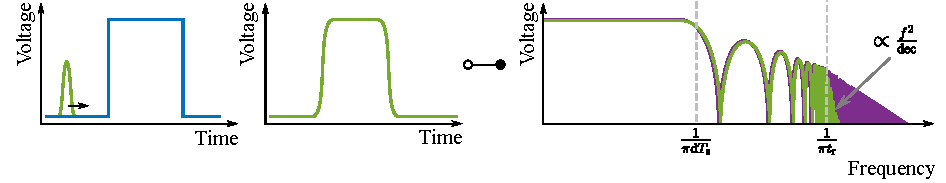
\includegraphics[scale = 1]{figures/2_Fundamentals/Diss_SpectrumCreation_Heisenberg.pdf}
	\caption{Graphical representation of the creation of the emission spectrum from a Gaussian approximation of the switching transient.}
	\label{fig:Diss_SpectrumCreation_Heisenberg}
\end{figure}

\subsubsection*{Simulated Spectra and the Need for Measurement}
\fref{fig:IntroFullSpec} shows the PSpice-simulated drain-source voltage of a hard-switched \SI{1200}{\volt} SiC MOSFET and its spectrum. Unlike the graphical approximations, the nonlinear device model captures switching transitions and circuit interactions, allowing comparison of the predicted envelope with the simulated spectrum.

\begin{figure}[ht]
	\begin{subfigure}{\textwidth}
		\centering
		\input{"figures/2_Fundamentals/DPT_TD_intro.tex"}
		\caption{PSpice-simulated drain-source voltage of a hard-switched SiC MOSFET.}
	\end{subfigure} %
	\par % Line break to stack subfigures
	\vspace{0.5cm}
	\begin{subfigure}{\textwidth}
		\hspace{-0.5cm}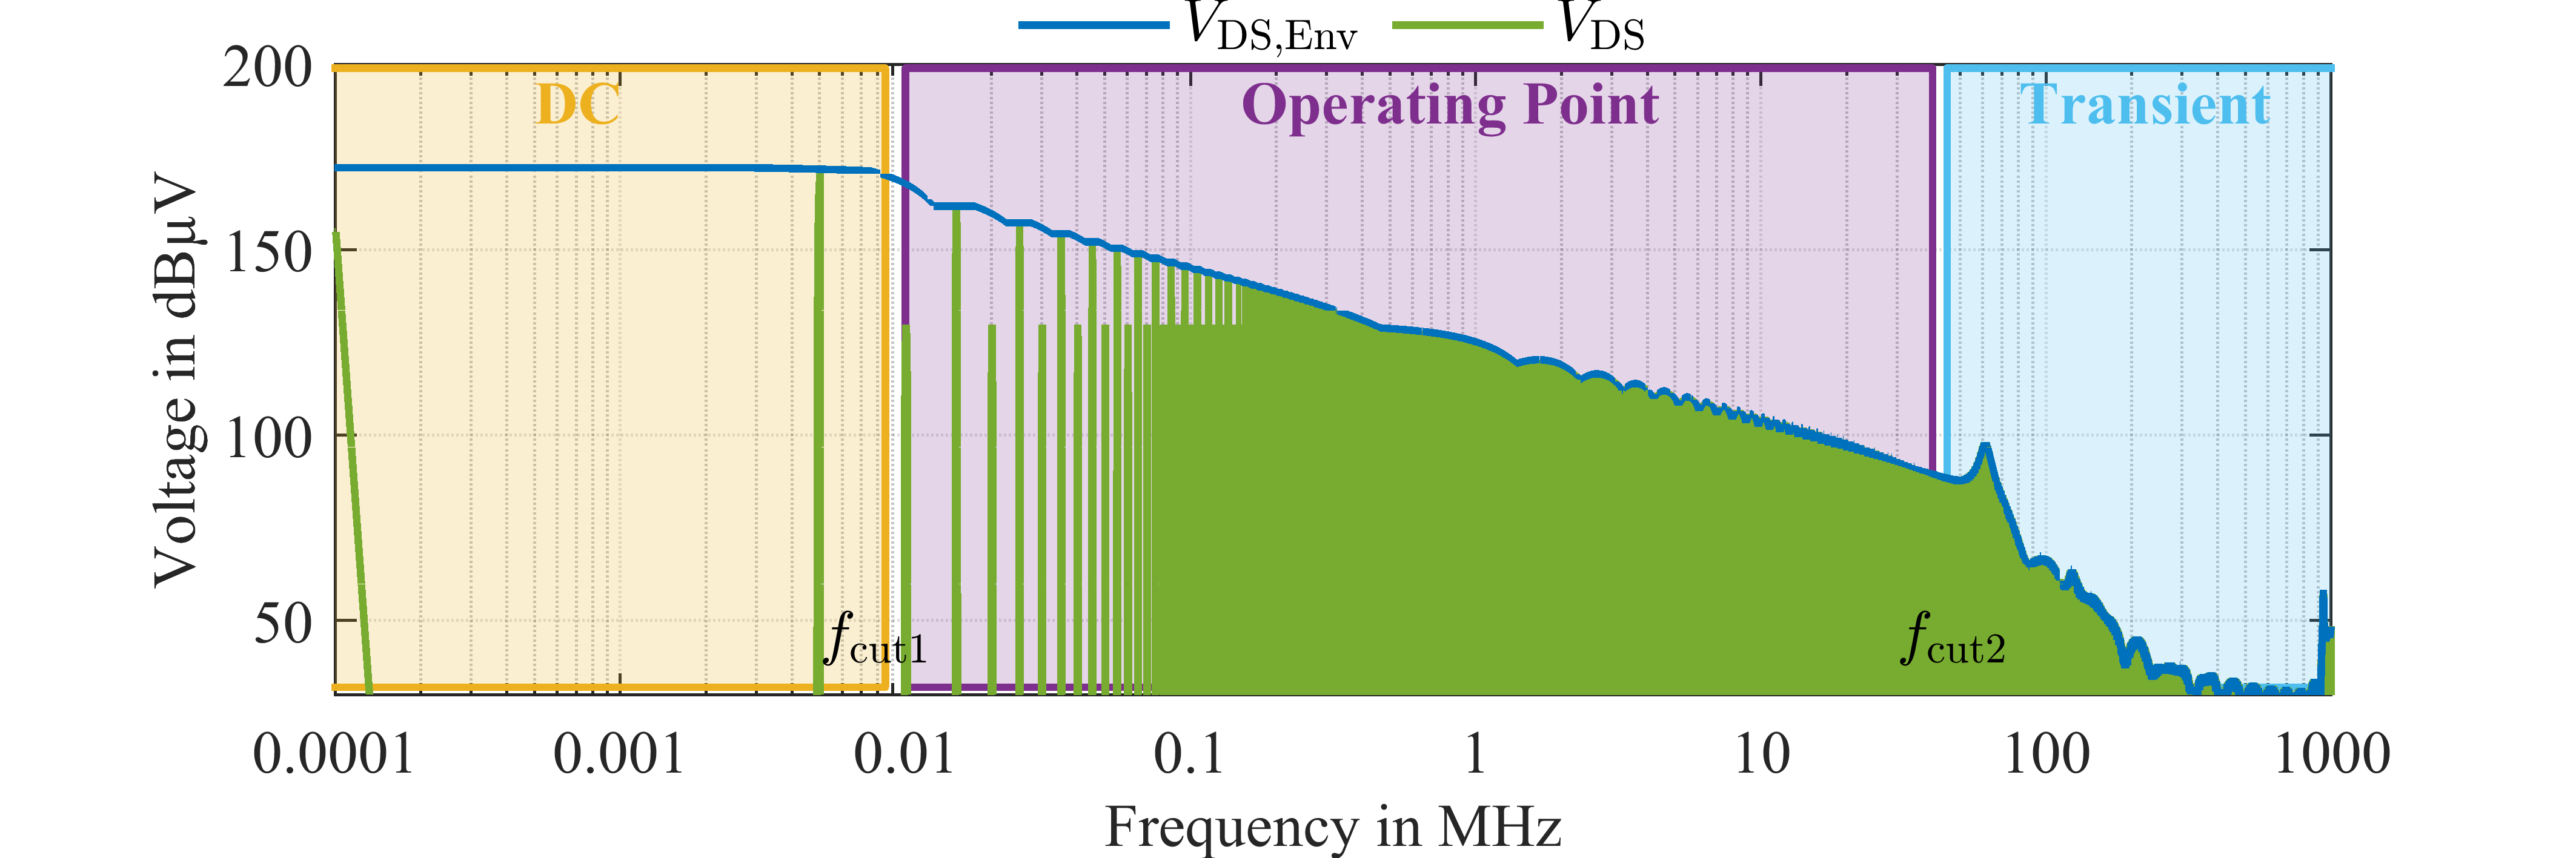
\includegraphics[scale = 1]{figures/2_Fundamentals/DPT_FD_intro.png}
		\caption{FFT of the simulated switching transient showing frequency regions dominated by different waveform phases.}
	\end{subfigure}
	\caption{Time-domain switching waveform and corresponding simulated voltage spectrum.}\label{fig:IntroFullSpec}
\end{figure}

Comparing the simulated spectrum with the graphical approximations shows that the rectangular-pulse model captures the low-frequency level and the approximately \SI{-20}{dB/dec} region. At higher frequencies, the spectrum departs from their constant-slope predictions as switching-edge details and circuit interactions become significant.

The regions labeled ``DC'', ``Operating Point'', and ``Transient'' in \fref{fig:IntroFullSpec} identify the dominant influences on different parts of the spectrum. 
The ``DC'' region is the low-frequency plateau, set by the DC-link voltage and duty cycle. In the ``Operating Point'' region, the switching frequency, duty cycle, and modulation strategy influence the spectrum. 
In the ``Transient'' region, the switching-edge duration and shape, together with associated oscillations, make the gate drive, device characteristics, and circuit parasitics important. 

\textbf{Limits of the Prediction:}
A physically plausible time-domain waveform does not establish the accuracy of its high-frequency spectrum, particularly above the dominant switching resonance.
The first limitation concerns model validation: calibration against conventional double-pulse measurements does not validate spectral components below the measurement noise floor, as discussed in the upcoming Section~\ref{sec:MeasurementLimitation}.
Agreement in switching time and overshoot can therefore coexist with substantial errors in much smaller high-frequency components.
The second limitation concerns numerical processing: solver tolerances, time steps and resampling all affect the computed spectrum.
Piecewise-linear interpolation, for example, can introduce derivative discontinuities and an artificial high-frequency tail.
The peak near \SI{900}{MHz} in \fref{fig:IntroFullSpec} illustrates the need to distinguish physical effects from numerical artifacts.
No physical mechanism could be identified to explain this peak, and it could be altered by changing the solver settings, indicating a numerical rather than a physical origin.
\\
\\
The graphical models provide a basis for interpreting the source spectrum, and simulation combines the underlying mechanisms within a circuit model.
Establishing the accuracy of the resulting predictions nevertheless requires measurements with sufficient bandwidth and dynamic range to resolve the relevant spectral components.
In the absence of a suitable measurement environment, none of the models considered here has yet been experimentally validated for predicting these small high-frequency spectral components.
Providing this experimental basis for model validation and the subsequent optimization of power-semiconductor switching behavior is a central aim of this thesis.

\FloatBarrier
\subsection{Propagation Paths in a Generic Inverter Application}
The switching transients discussed above excite noise currents that propagate through the inverter and its connected components to the external system ports.
The resulting conducted emissions depend on both the semiconductor switching behavior and the impedances of these propagation paths.
Although filtering and careful layout can reduce the coupling to external systems, complete suppression over the entire frequency range is not practically achievable.
% Characterizing the noise source therefore remains essential for understanding and mitigating system-level emissions.

\fref{fig:ESB_CMDM_Propagation} shows a simplified equivalent circuit for one phase of a three-phase machine inverter.
The circuit comprises an inverter half-bridge, the DC supply cables, and a machine represented by its winding impedance, the back electromotive force induced by rotor rotation, and parasitic capacitances to ground.
In an electric vehicle, this ground reference typically corresponds to the chassis rather than either DC supply conductor.
A line impedance stabilization network (LISN) is inserted between the power supply and the inverter to establish a defined impedance within the specified measurement band and to attenuate disturbances from the supply.
In the illustrated equivalent circuit, the LISN is represented by a $\pi$-type filter with a series inductor and shunt capacitive branches.
The inverter-side series $RC$ branch forms part of the low-impedance path for high-frequency disturbances. 
The measurement port is incorporated into this path, and the voltage across its termination resistance is measured.
This voltage is related to the noise current through the LISN transfer impedance; it is not a direct measurement of the total chassis current.

\begin{figure}[h]
	\centering
	\import{./figures/2_Fundamentals/}{Diss_ESB_CMDM_Propagation.pdf_tex}
	\caption{Equivalent circuit of the common-mode and differential-mode noise propagation paths.}
	\label{fig:ESB_CMDM_Propagation}
\end{figure}

The conducted noise currents at the LISN ports can be decomposed into differential-mode (DM) and common-mode (CM) components.
DM currents flow in opposite directions in the two supply conductors and close their loop through the power circuit.
CM currents, by contrast, flow in the same direction in both supply conductors and therefore require a ground return path. 


For the modal decomposition, \mi{I}{LISNp} and \mi{I}{LISNn} denote the noise currents in the positive and negative supply conductors at the LISN interface, respectively. 
The DM and CM components are then defined as
\begin{equation}
	\mi{I}{DM} = \frac{\mi{I}{LISNp} - \mi{I}{LISNn}}{2}
\end{equation}
and
\begin{equation}
	\mi{I}{CM} = \frac{\mi{I}{LISNp} + \mi{I}{LISNn}}{2}.
\end{equation}
With this convention, \mi{I}{CM} is the common-mode component per conductor.
Because the decomposition involves adding and subtracting the two currents, their relative timing or phase must be retained.
The equations therefore apply to instantaneous currents or complex frequency-domain quantities, not two independently measured spectral magnitudes.


Differential-mode currents are high-frequency components superimposed on the load current.
As the semiconductor devices switch, they draw pulsed current from the DC link.
The finite impedance of the DC-link capacitor allows this current to produce voltage fluctuations across the capacitor, which in turn drive the differential-mode current flowing in the supply conductors.

Switching transitions also excite common-mode currents, which flow through parasitic capacitances between circuit nodes and the chassis.
The parasitic capacitances \mi{C}{DC+} and \mi{C}{DC-} couple the positive and negative DC rails to ground, while \mi{C}{SwN} and \mi{C}{SP} represent the ground coupling of the switching node and the machine star point, respectively.
Changes in the voltage across these capacitances drive displacement currents according to $i_C = C\,\sddt{v}$.
These currents must return to their sources through the lowest-impedance path.
In an unfiltered setup, the return path may run through the chassis, the LISN, and the supply cables back to the inverter.
Y-capacitors, DC filters, and the design of the power cables can be used to shape this path in applications.

Which common-mode coupling path dominates depends strongly on the application.
The switching node experiences the highest voltage slew rate and is directly coupled to the chassis through \mi{C}{SwN}.
Although this capacitance is typically much smaller than the star-point capacitance, the high \sddt{v} can still produce a substantial displacement current.
The star-point capacitance is typically larger, but the voltage slew at the star point is reduced by capacitive voltage division across the motor winding capacitances.
Consequently, the larger capacitance does not necessarily produce a larger common-mode current.

The contributions of \mi{C}{DC+} and \mi{C}{DC-} to the common-mode current also depend on the commutation-loop design.
For example, when the DC rails have equal impedances and equal parasitic capacitances, their voltages vary in opposite directions relative to ground, causing the resulting ground-current contributions to cancel.
In coplanar designs, the parasitic capacitances of the two DC rails can be strongly asymmetric, increasing their net contribution to the common-mode current.
However, coplanar layouts also shield the switching node, reducing its coupling to the chassis and the contribution of \mi{C}{SwN}.
Overall, this shielding results in lower common-mode emissions in coplanar designs.

In addition to conducted emissions, the commutation loop also produces radiated emissions: its fast changing voltages and currents generate electric and magnetic fields that propagate through space.
Because no enclosure provides perfect shielding, some of these fields can escape through apertures and connectors.
Radiated emissions are particularly relevant above \SI{108}{\mega\hertz} and are typically measured in a shielded EMC chamber.

Because propagation paths strongly influence both conducted and radiated emissions, considerable research has addressed their characterization and mitigation.
This thesis, however, focuses on noise generation rather than on propagation and mitigation strategies.

\subsection{From Switching Sources to System-Level Emissions}


\begin{figure}
	\begin{subfigure}[t]{0.48\textwidth}
		\centering
		\raisebox{7mm}{\import{./figures/}{1_Introduction/NoiseGenerationSystem/DPT_TD.tex}}
		\subcaption{Drain-source voltages of the active and passive devices.}
		\label{fig:SourceToSystem_TD}
	\end{subfigure}
	\hfill
    \begin{subfigure}[t]{0.48\textwidth}
		\centering
		% \import{./figures/}{Snap_n_Mirror_vertical_v3_tex.pdf_tex}
		\import{./figures/}{GenerationVSpropagation_Converter.pdf_tex}
		\subcaption{Simplified equivalent circuit of the half-bridge converter.}
		\label{fig:SourceToSystem_Circuit}
	\end{subfigure}

	\vspace{0.5cm}
	\begin{subfigure}[t]{0.48\textwidth}
		\centering
		\import{./figures/}{1_Introduction/NoiseGenerationSystem/DPT_FD.tex}
		\subcaption{Voltage spectra of the active and passive devices.}
		\label{fig:SourceToSystem_Spectra}
	\end{subfigure}
	\hfill
	\begin{subfigure}[t]{0.48\textwidth}
		\centering
		\import{./figures/}{1_Introduction/NoiseGenerationSystem/TF_FD.tex}
		\subcaption{Artificial transfer functions from the devices to the LISN measurement port.}
		\label{fig:SourceToSystem_Transfer}
	\end{subfigure}
    
	\vspace{0.5cm}
    \begin{subfigure}[t]{0.98\textwidth}
		\centering
		\import{./figures/}{1_Introduction/NoiseGenerationSystem/System_FD.tex}
		\subcaption{Individual contributions and total LISN voltage spectrum with a emission limit. The limit is hypothetical and does not represent a CISPR compliance assessment.}
		\label{fig:SourceToSystem_LISN}
	\end{subfigure}
	\caption{Illustration of how switching noise sources and their propagation paths combine to shape the system-level emissions of a half-bridge converter, using simulated waveforms and artificial transfer functions.}
	\label{fig:SourceToSystem}
\end{figure}

The preceding subsections considered the generation and propagation of electromagnetic disturbances separately.
\fref{fig:SourceToSystem} combines these two aspects to illustrate how the switching waveforms of a half-bridge converter contribute to the voltage spectrum at a LISN measurement port.
The example uses simulated switching waveforms and artificial transfer functions to demonstrate the interaction between the noise sources and their propagation paths, rather than to predict the emissions of a specific prototype.



\fref{fig:SourceToSystem_TD} shows the drain-source voltages of the actively switched device and the complementary, passively commutated device.
Their different transition shapes and oscillations produce the source spectra shown in \fref{fig:SourceToSystem_Spectra}.
These spectra describe the disturbances at the devices, but do not directly indicate their contributions at the LISN measurement port.
As illustrated by the equivalent circuit in \fref{fig:SourceToSystem_Circuit}, each source is coupled to the measurement port through a different path.

The corresponding transfer functions in \fref{fig:SourceToSystem_Transfer} describe how strongly each frequency component is transmitted to the LISN measurement port.
Multiplying each complex source spectrum by its transfer function gives its contribution to the port voltage.
The total voltage is then obtained by adding these contributions with their relative phase retained.


\fref{fig:SourceToSystem_LISN} shows the individual contributions and the resulting LISN voltage spectrum.
The frequency dependence of the propagation paths changes the relative importance of the two sources and introduces spectral peaks and attenuation.
Consequently, a prominent feature at the measurement port need not correspond to a prominent feature in either source spectrum alone.
Reducing system-level emissions therefore requires considering both the switching behavior and the paths through which its disturbances propagate.
Whether the resulting emissions are acceptable is assessed using standardized measurement procedures and limits, introduced in the following subsection.

\FloatBarrier

\subsection{Standardized EMC Measurements and Limits}
Standardized emission measurements provide reproducible conditions for assessing the disturbances generated by a device under test (DUT).
CISPR, the International Special Committee on Radio Interference within the International Electrotechnical Commission (IEC), develops standards for such measurements and their limits.
For automotive applications, CISPR~25 specifies methods and limits for conducted and radiated disturbances.
The CISPR~16 series provides basic specifications for measuring apparatus and measurement methods, which are referenced where applicable by product standards.

Conducted emission measurements assess disturbances coupled into the connected wiring.
In the voltage method, a LISN establishes a defined supply impedance and couples the disturbance voltage to a measurement receiver.
Radiated emission measurements instead use antennas to measure the electromagnetic field produced by the DUT and its wiring under specified test conditions.
The antenna type, position, and polarization, together with the arrangement of the DUT and cables, are prescribed to obtain reproducible results.

In many EMC test schemes, conducted emissions are assessed up to \SI{30}{\mega\hertz}, while radiated measurements cover higher frequencies into the gigahertz range.
This division is not universal: the applicable frequency ranges depend on the product standard and measurement method, and automotive conducted-emission tests can extend beyond \SI{30}{\mega\hertz}.

Automotive inverter and converter suppliers may also be required to meet customer-specific conducted-emission limits up to \SI{100}{\mega\hertz} or higher.
Such requirements can supplement standardized tests with additional frequency ranges or stricter limits defined by the vehicle manufacturer rather than by the standard itself.
Their purpose is to reduce interference risks during component integration and to provide margin for the final vehicle-level EMC assessment.
Compliance at component level therefore supports, but does not guarantee, compliance of the complete vehicle, whose emission behavior also depends on the installed wiring and interactions between components.

The measured levels are compared with frequency-dependent limits for the applicable test method and limit class.
These limits must be used together with the specified receiver bandwidth and detector, such as peak, quasi-peak, or average, as applicable.
A simulated FFT spectrum cannot therefore be compared directly with a compliance limit unless the measurement conditions and receiver response are represented consistently.
The hypothetical limit in \fref{fig:SourceToSystem_LISN} is a simplification and is not taken from a standard: the figure shows the total LISN voltage \mi{V}{LISN}, whereas conducted-emission limits are specified separately for DM and CM measurements.
